\documentclass[12]{article}
\usepackage[margin=1.0in]{geometry}
\usepackage[utf8]{inputenc}
\usepackage{titlesec}
\usepackage{physics}
\usepackage{graphicx}
\usepackage{siunitx}
\usepackage{cancel}
\usepackage{amsmath}
\usepackage{textcomp}
\usepackage{gensymb}
\usepackage{natbib}
\usepackage{bm}
\usepackage{setspace}
\usepackage[version=4]{mhchem}

\titleformat*{\subsection}{\normalfont\fontfamily{phv}}
%\titleformat*{\subsection}[runin]{}{}{}{}[]
  \titleformat{\subsection}[runin]{\normalfont\bfseries}{\thesubsection.}{3pt}{}
  \titleformat{\subsubsection}[runin]{\normalfont\bfseries}{\thesubsubsection.}{3pt}{}

\title{{\textsc{\Large Antarctic Radiative and Temperature responses to a doubling of $\text{CO}_2$}}}
\author{\textsc{Lyssa Freese}
\\\\
Advised by Prof. Tim Cronin}
\doublespacing
\begin{document}
\maketitle
\thispagestyle{empty}

\setlength{\leftskip}{1.1cm}
\setlength{\rightskip}{1.1cm}


\bigskip
\bigskip

{\textsc{Abstract.} }
Greenhouse gases (GHGs), such as \ce{CO2}, impact global and local outgoing longwave radiation (OLR). The Antarctic is known for its a strong near-surface temperature inversion, where the addition of GHGs can lead to increased OLR due to higher radiating temperatures higher in the atmosphere. Here we develop a radiative-advective-turbulent single-column model based on observed temperatures at the South Pole and timestep it forward under different \ce{CO2} concentrations. We discuss 1) radiative diagnostics of the observed temperature profiles under varying \ce{CO_2} concentrations and 2) variation of temperature and radiative fluxes as we timestep the model forward to equilibrium under a normal and doubled \ce{CO_2} scenario. We confirm previous results showing negative top-of-atmosphere forcing with increased \ce{CO_2} during all seasons but austral winter. Despite this negative forcing, we find increased temperatures at the surface across all seasons and cooling in the stratosphere with a doubling of \ce{CO_2}.
\bigskip
\bigskip 
\clearpage
\setcounter{page}{1}

\setlength{\leftskip}{0cm}
\setlength{\rightskip}{0cm}

\section{Introduction}
The Antarctic is characterized by a strong, year-round temperature inversion in the bottom 1 km of the atmosphere: surface temperatures, particularly in the central part of the continent, are colder than atmospheric temperatures just above them \citep{hudson_look_2005}. As emissions of \ce{CO_2} continue to rise due to anthropogenic sources \citep{peters_carbon_2020}, the role that greenhouse gases (GHGs) play in local Antarctic radiative balance, where such a temperature inversion is present, are important to consider. Near surface air temperatures under increasing levels of GHGs are important to understand for their role in ice sheet stability and thus sea level rise \citep{hanna_ice-sheet_2013}. 

Previous work has found that increasing GHG concentrations in the Antarctic results in a negative greenhouse effect due to an increase in OLR \citep{schmithusen_how_2015}. This was seen in a two-layer model, line-by-line radiative transfer calculations, and experiments with the European Centre for Medium-Range Weather Forecast (ECMWF) atmospheric model. These conclusions; however, do not describe the impact that GHG have on surface temperature or the structure of the atmospheric column temperature. In order to investigate the implications that chlorofluorocarbons (CFCs) would have in the Antarctic, \cite{flanner_climate_2018} utilize the Community Earth System Model (CESM), a fully coupled atmosphere, ocean, and land model, to model the surface and atmospheric temperature response. This work finds warming surface temperatures, and cooling in the layer in which CFCs were added. Theoretical work utilizing a grey gas model similarly found increasing surface temperatures in response to increased optical depth in a high latitude scenario \citep{payne_conceptual_2015}.

We aim to bring together much of this work by developing a single-column radiative-advective-turbulent equilibrium (RATE) model rooted in observations, in order to build upon the theoretical findings in high latitude scenarios. The model has these three terms to allow for an equilibrium state in which advective heating in the winter and shortwave heating due to absorption by ozone in the summer balance longwave cooling. Advection is included to represent meridional heat transport of warm air from lower latitudes to the South Pole, similar to the idealized radiative advective model proposed in \cite{cronin_analytic_2016}. We build on this idealized model by also including an exponentially decaying turbulent component, which is meant to represent turbulence in the planetary boundary layer. We conduct a diagnostic analysis of the radiative fluxes that result from the observed temperature profiles in our initial state and run them to equilibrium in our RATE model to see how \ce{CO_2} affects the equilibrium state. We find that 1) OLR responses are dependent upon season, 2) surface net longwave fluxes decrease with increasing GHG concentration, 3) and that surface temperature and OLR increase after five months under higher GHG concentrations, despite the initial negative greenhouse effect.


\section{Methods}

\subsection{Temperature and gas data}
 To create monthly column gas and temperature profiles (Figure \ref{fig:temperature_profiles}), we utilize monthly-average temperature profiles from the South Pole station, modified according to \cite{schmithusen_how_2015}, as well as yearly average ozone volumetric mixing ratio (vmr), and water vapor vmr (w) \citep{schmithusen_how_2015}. The column specific humidity is calculated at every level using
\begin{equation}
    q = w/(1+w).
\end{equation}

\begin{figure}[htb!]
\noindent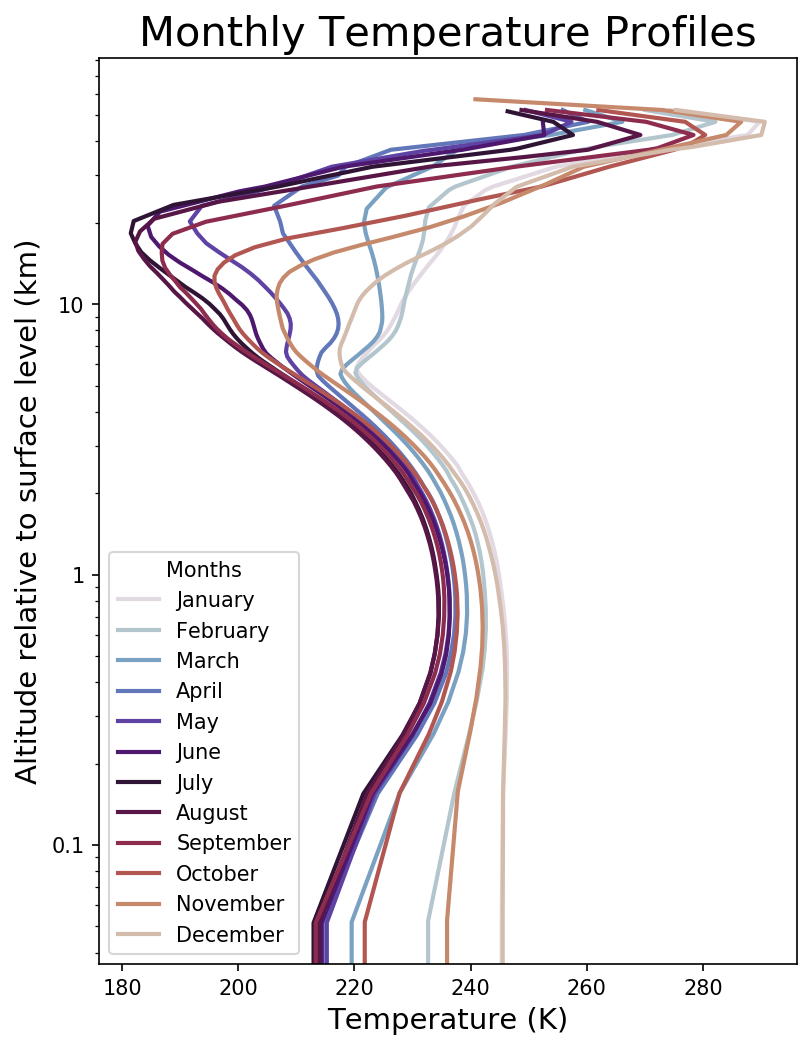
\includegraphics[width=.5\textwidth]{figures/initial_temperature_profiles.png}
\centering
\caption{Initial monthly temperature profiles based on a combination of radiosonde observational data and reanalysis (for the stratosphere). Winter months have sharper temperature inversions due to decreased shortwave radiation.}
\label{fig:temperature_profiles}
\end{figure}

 We adjust the lowest levels of the temperature, ozone, and specific humidity profiles to coarsen the vertical resolution to about 100 m, which ensures that we satisfy the CFL condition $\frac{k_0 \Delta t}{\Delta z^2_{surf}} < 1$ for a timestep of $\Delta t =$ one hour (see set-up of turbulence model below). A range of well-mixed column CO2 profiles are created, from 0 to 1500 ppm, in order to give a full range of responses to different values. We utilize 380ppm as our base-case, and 760ppm as a doubled-\ce{CO_2} case for the equilibrium state of the model.

\subsection{Model Setup}
We utilize these monthly temperature profiles in a single column model in CLIMLAB \citep{rose_climlab_2018}, an open source climate model in Python. We adjust the solar insolation to a monthly mean insolation, to capture the large variability in shortwave radiation between summer and winter seasons in the Antarctic (insolation values can be seen in Figure \ref{fig:solar_insol}).

\begin{figure}[htb!]
\noindent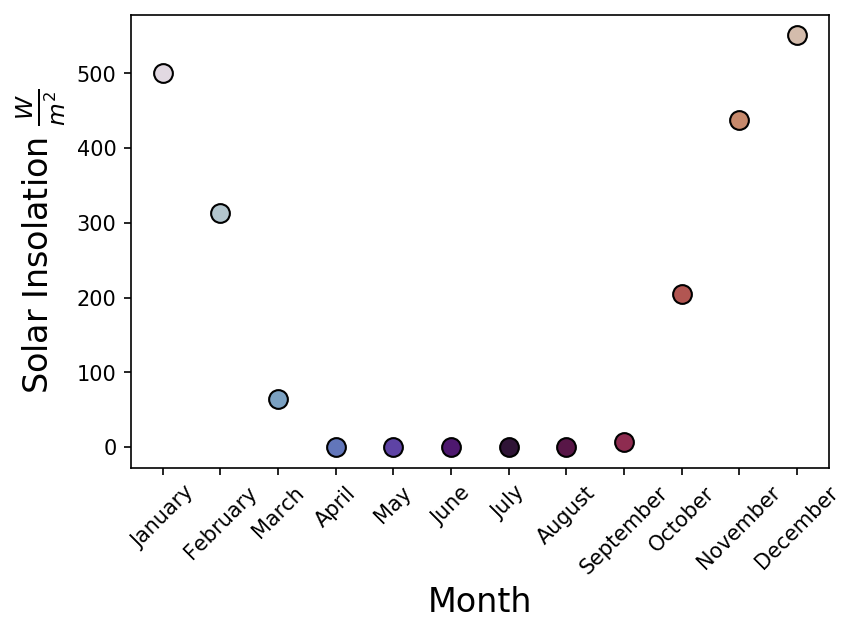
\includegraphics[width=.5\textwidth]{figures/solar_insol.png}
\centering
\caption{Monthly solar insolation, which decreases sharply to near-zero values in the winter months.}
\label{fig:solar_insol}
\end{figure}

RATE is comprised of three parts: a radiative component, an advective component, and a turbulent component. The model computes temperature tendencies from the flux divergence of each component and steps the temperature forward in time according to:
\begin{equation}
    \rho c_{p} \pdv{T}{t} = -\nabla \cdot \mathbf{\mathcal{F}}
\end{equation}

\subsubsection{Radiation}
The radiation is calculated utilizing the RRTMG radiation scheme \citep{mlawer_radiative_1997} such that 

\begin{equation}
    \text{HR}_{\text{rad}} = -\frac{\text{dF}_{\text{rad}}}{dz} /(c_p \rho) \quad \text{for both shortwave and longwave fluxes}
\end{equation}
RRTMG calculates absorption and emission in wavelength bands for our prescribed values \ce{N_2O}, \ce{CH_4}, \ce{O_2}, \ce{CO_2}, and ozone, all of which are assumed to be well mixed except for ozone, which has prescribed values at each pressure level.

\subsubsection{Turbulence}
We construct a near-surface turbulence component based on the turbulent flux of potential temperature
\begin{equation}
    F_{turb} = -k(z) \frac{d\theta}{dz},
\end{equation}
where $k(z) = \overline{k_0} \exp(-\frac{z}{d})$ is an exponentially decaying diffusivity with a surface value of $k_0$ and a turbulence scale factor of $d = 100$ meters, which confines substantial turbulent fluxes to the bottom few model levels. We calculate $k_0$ diagnostically from the initial condition
\begin{equation}
    k_0^{(m)} = \frac{F_{\text{sfc, rad}}}{\frac{d\theta}{dz}_{\text{sfc}}},
\end{equation}
for each month $m$, where our radiative surface flux is calculated as
\begin{equation}
    F_{\text{sfc, rad}} = F_{\text{sfc, SW}} - F_{\text{sfc, LW}}.
\end{equation}

From this, we average the (nine) positive $k_0^{(m)}$ values, and use this as our final $\overline{k_0}$ throughout the experiments.

The turbulent heating rate is thus the flux divergence divided by the heat capacity of air and ice, for the atmosphere and surface, respectively:
\begin{equation}
    \text{HR}_{\text{turb}} = -\frac{\text{dF}_{\text{turb}}}{dz} /(c_p \rho).
\end{equation}

Our turbulence profiles vary across months, warming the surface during the winter and cooling it in the summer in order to balance the surface radiative heating rates.

\subsubsection{Advection}
We calculate our advective heating rate based on the initial state for each month at \ce{CO_2} = 380ppm, where it is set to balance the sum of the radiative and turbulent heating rates.

\begin{equation}
    \frac{dF_{adv}}{dy} = -(\frac{dF_{rad}}{dz} + \frac{dF_{turb}}{dz})\quad \text{at t = 0 and \ce{CO_2} = 380 ppm}
\end{equation}
The resulting advective heating rate is held constant throughout time, in order to allow us to isolate the adjustments of the radiative and turbulent components in time. 
We run the model forward for five months to assess the equilibrium state in our base case and doubled \ce{CO_2} scenarios. We focus on the months of December and June to represent the austral summer and winter, respectively.

\section{Results}
\subsection{Initial State}
In our initial state (Figure \ref{fig:temperature_profiles}), we see a clear temperature inversion in the bottom $1$ km, as expected, across all months \citep{connolley_antarctic_1996}. This inversion is stronger during the austral winter when surface warming from shortwave radiation is at a low. 

The initial conditions under each of our column \ce{CO_2} concentrations show variations in OLR, surface net longwave flux, and surface net shortwave flux. For \ce{CO_2} concentrations above 100 ppm, OLR increases with atmospheric \ce{CO_2} concentration in December, but decreases with \ce{CO_2} concentrations in June (Figure \ref{fig:init_OLR}). This decreasing trend is evident across May-August, while the rest of the year exhibits increases in OLR with increased \ce{CO_2}. This is in line with the conclusions of previous work, which finds positive radiative forcing by \ce{CO_2} and thus decreasing OLR during the winter \citep{schmithusen_how_2015}. This increase in OLR with increasing \ce{CO_2} concentrations leads to increasing top-of-atmosphere (TOA) radiative loss under higher GHG scenarios during September-April. 

\begin{figure}[htb!]
\noindent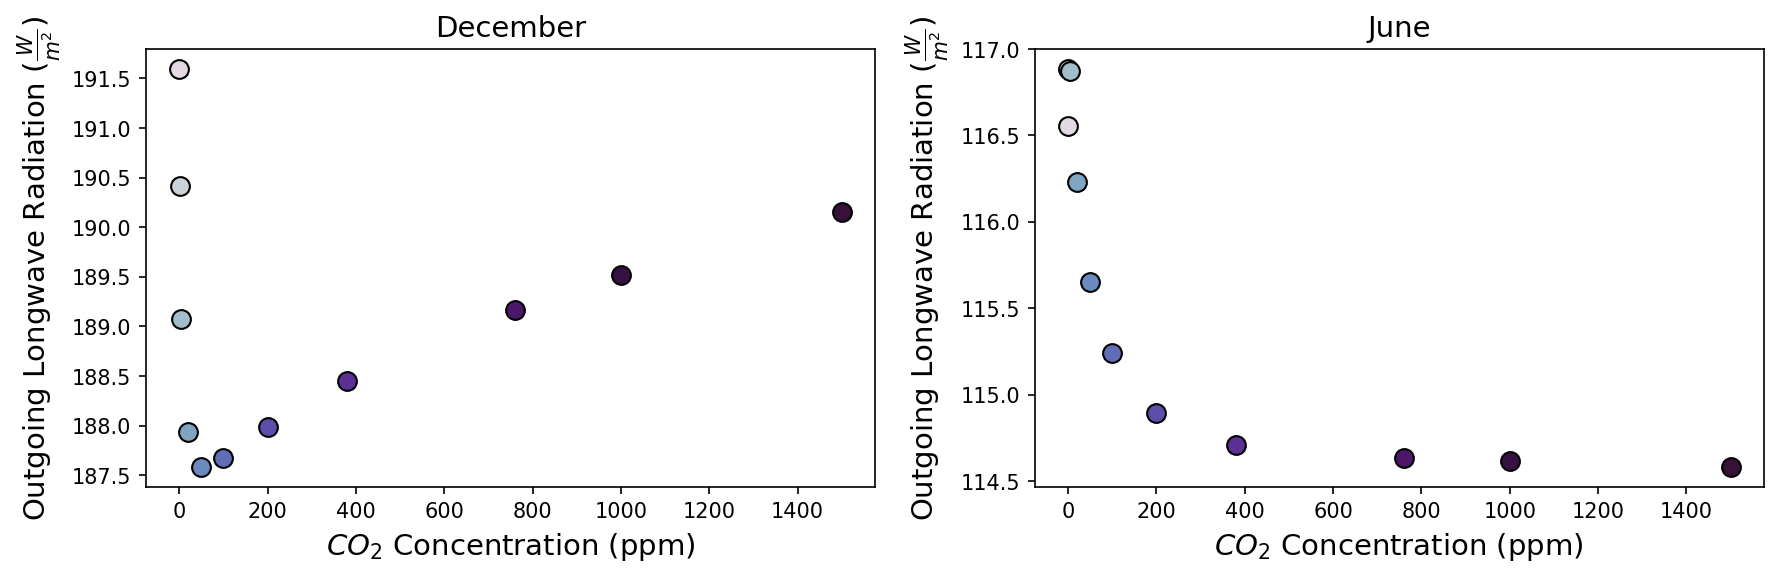
\includegraphics[width=1\textwidth]{figures/OLR_init.png}
\centering
\caption{Initial OLR calculated at different \ce{CO_2} levels in June and December. The December case shows increasing OLR with concentration, while June has decreasing OLR with concentration.}
\label{fig:init_OLR}
\end{figure}

\begin{figure}[htb!]
\noindent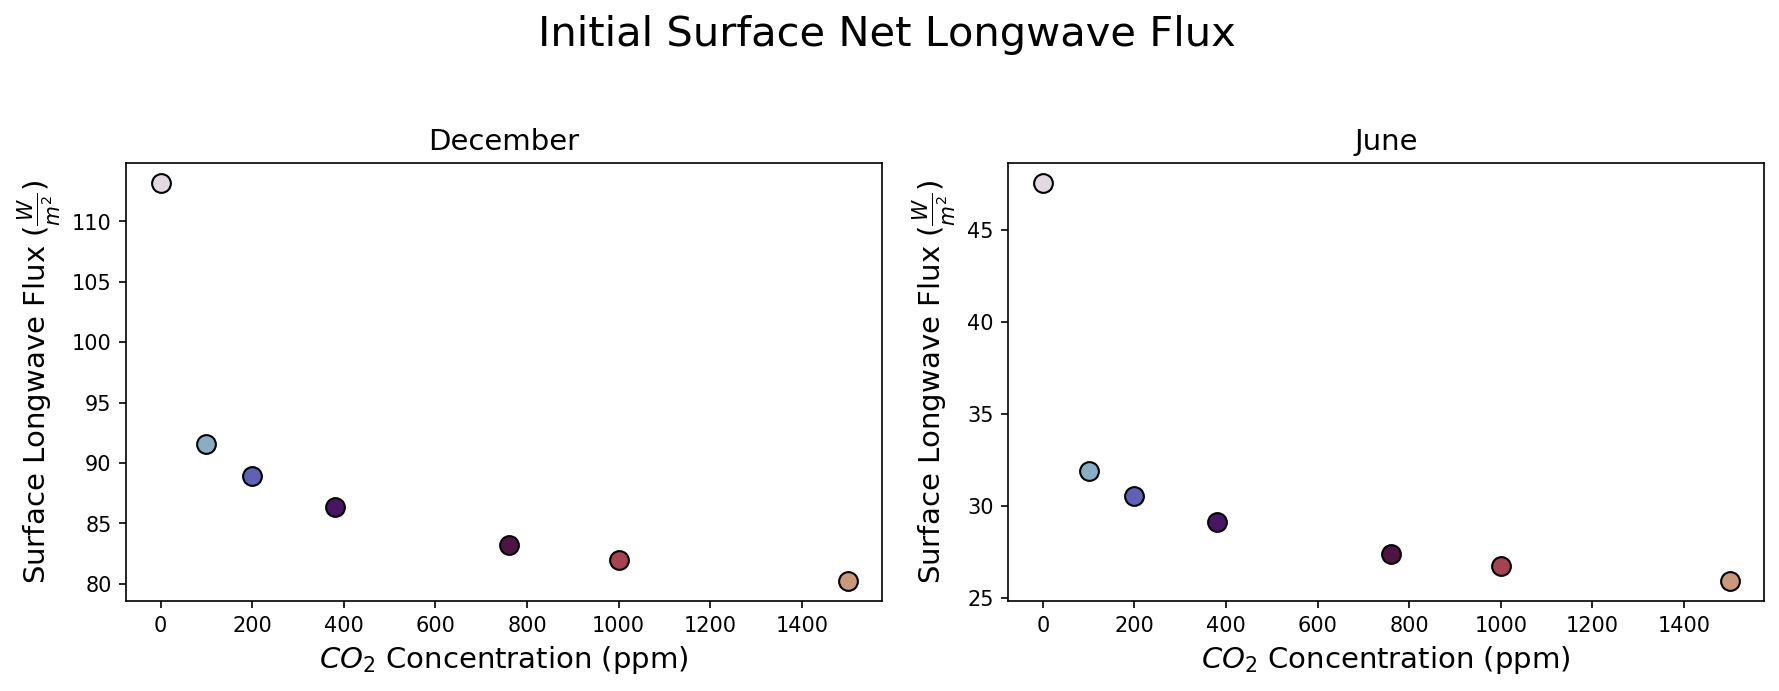
\includegraphics[width=1\textwidth]{figures/sfcLW_init.png}
\centering
\caption{Initial surface net longwave radiation calculated at different \ce{CO_2} levels in June and December. Both months show decreasing surface net longwave with increased \ce{CO_2} concentrations.}
\label{fig:init_sfc_LW}
\end{figure}

We find the initial surface net longwave flux decreases with increasing \ce{CO_2} levels across both summer and winter months. In the summer, the net surface shortwave flux also slightly decreases, due to an increase in \ce{CO_2} absorption in the shortwave.  The initial surface upward longwave fluxes $\sigma T_s^4$ are the same across \ce{CO_2} concentrations, since the surface temperatures ($T_s$) only vary by month. Thus the surface downward longwave flux is what contributes to the changing net flux, as it increases with a higher optical thickness, and the temperature and level from which it is radiating downwards is closer to the ground at a higher \ce{CO_2} concentration. The surface downward shortwave flux and upward shortwave flux are both impacted by \ce{CO_2} concentration and optical thickness, in which downward flux is increased, and upward flux is decreased, but the overall change is much smaller than for the longwave, because \ce{CO_2} mostly intersects with the longwave infrared (IR) spectra, but has small absorptivity in the shortwave IR range in the RRTMG model (at wavenumbers between 2380-2600 cm$^{-1}$ \citep{mlawer_radiative_1997}. 

Additionally, we estimate the greenhouse effect (GHE) of \ce{CO_2} at our initial timestep for each month (Figure \ref{fig:GHE}). We calculate this for a given month (m) and \ce{CO_2} concentration (c) as
\begin{equation}
    \text{GHE} = \text{OLR}_{c=0}^{(m)} - \text{OLR}_{c}^{(m)}
\end{equation}

We find similar results to that of \citep{schmithusen_how_2015}, in which our February, March and April GHE are negative across all \ce{CO_2} concentrations, and October and September shift from an initial positive GHE to negative as concentrations increase. During both spring and fall months we see the strongest cooling effect of \ce{CO_2}, and overall, the GHE in Antarctica is far smaller than for a standard atmosphere \citep{schmithusen_how_2015}.

\begin{figure}[htb!]
\noindent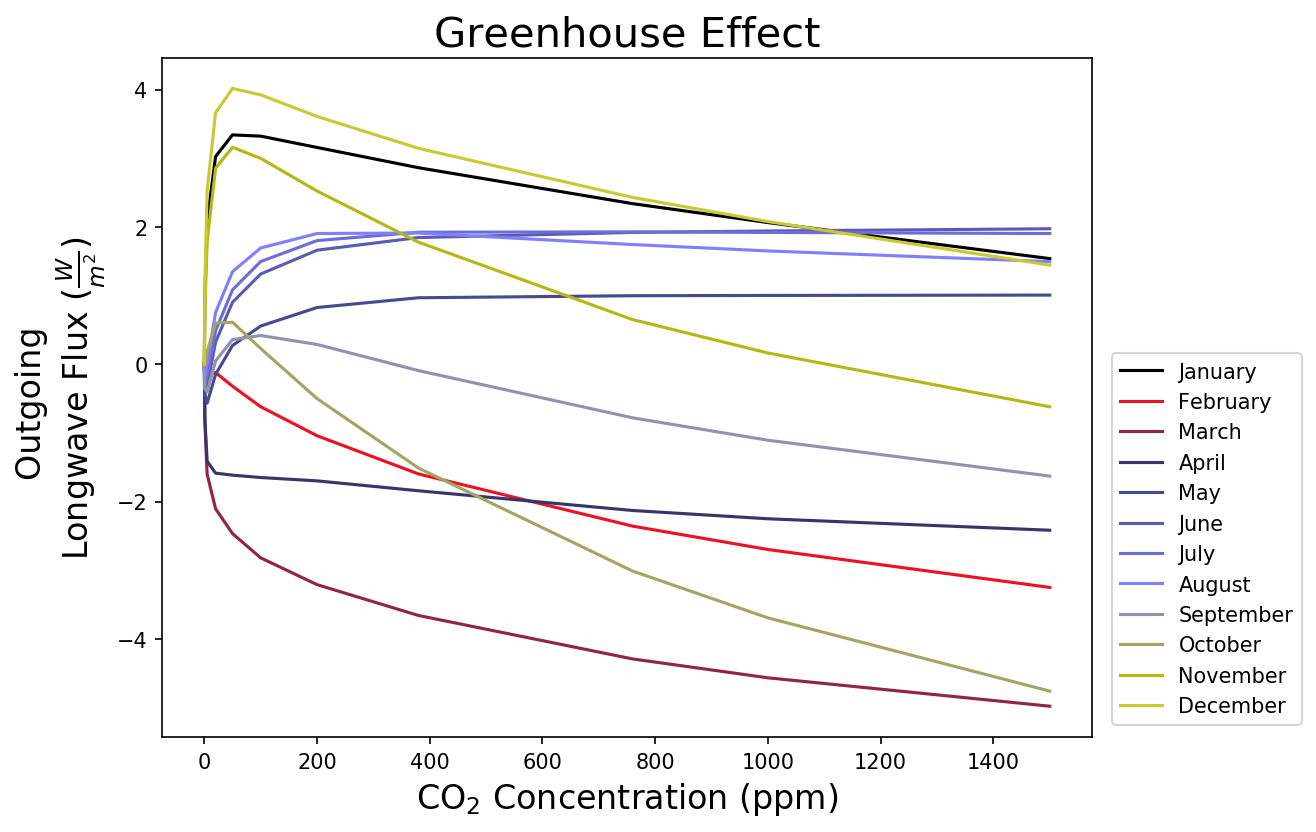
\includegraphics[width=.8\textwidth]{figures/GHE.png}
\centering
\caption{Greenhouse effect of \ce{CO_2} values for each month.}
\label{fig:GHE}
\end{figure}

\subsection{Change over time}
Here we look at the impacts of \ce{CO_2} concentration and season after running the model forward for five months to an equilibrium state. 

The sum of the column integrated advection for a given month and \ce{CO_2} concentration with the ASR at a given timestep should equal the OLR at an equilibrium state,
\begin{equation}
    \text{OLR}^{(m)}_{c}(t) = \text{ASR}^{(m)}_{c}(t) +  \int_{z=0}^{\text{TOA}}{\text{F}_{\text{adv}}^{\text{(m,z,c)}} c_p \rho^{\text{(m,z,c)}} dz},
\end{equation}
where $c$ is the \ce{CO_2} concentration, $m$ is the month, and $z$ is the altitude, which is what we see our model moving towards in Figure \ref{fig:ASR_OLR}. 

In order to reach an equilibrum, the OLR increases in order to match the sum of ASR and advection. The OLR in June between the base and double \ce{CO_2} scenarios are equivalent because the ASR is close to zero, and advection is held constant (with only slight changes in column integrated values over time as the density of the atmosphere shifts with changing temperatures). In the case of December, there are slight differences in our base and double \ce{CO_2} scenario OLR due to changes in ASR associated with different atmospheric \ce{CO_2} concentrations. This is in contrast to the initial state, in which the differences in OLR were due to diagnostic calculations of OLR at a given \ce{CO_2} concentration.

\begin{figure}[htbp!]
\noindent
\includegraphics[width=1\textwidth]{figures/ASR_OLR.png}
\centering
\caption{Evolution of OSR in comparison to ASR plus column integrated advection in both the base case and double \ce{CO_2} case for December and June. Differences in OLR at the equilibrium state are due to differences in ASR. Differences between OLR and the ASR plus column integrated advection indicate that the model is not at a complete equilibrium.}
\label{fig:ASR_OLR}
\end{figure}

In this case where the OLR are approximately the same for a base and double \ce{CO_2} case, there will be impacts on the temperature structure of the atmosphere. Our surface (and tropospheric) temperature increases more under the double \ce{CO_2} case because an increase in \ce{CO_2} leads to a lower pressure from which the atmosphere is radiating to space. This lower pressure level is associated with a lower temperature, but in order to keep the OLR the same, the temperature at this pressure level has to increase. In the stratosphere, an increase in \ce{CO_2} and the subsequent shift in pressure levels radiating to space lead to a higher radiating temperature. In order to keep OLR the same, the radiating temperature must decrease. The stratospheric cooling offsets the tropospheric warming due to doubled \ce{CO_2}, while maintaining a constant OLR. As we have kept advection equivalent across all timesteps and \ce{CO_2} concentrations (varying it only by month), the cooling seen throughout the stratosphere in the doubled \ce{CO_2} case is due specifically to radiative forcing by \ce{CO_2}. The stratospheric cooling we find is in line with typical responses to \ce{CO_2} increases \citep{rind_climate_1989, fels_stratospheric_1980}. 

\begin{figure}[htbp!]
\noindent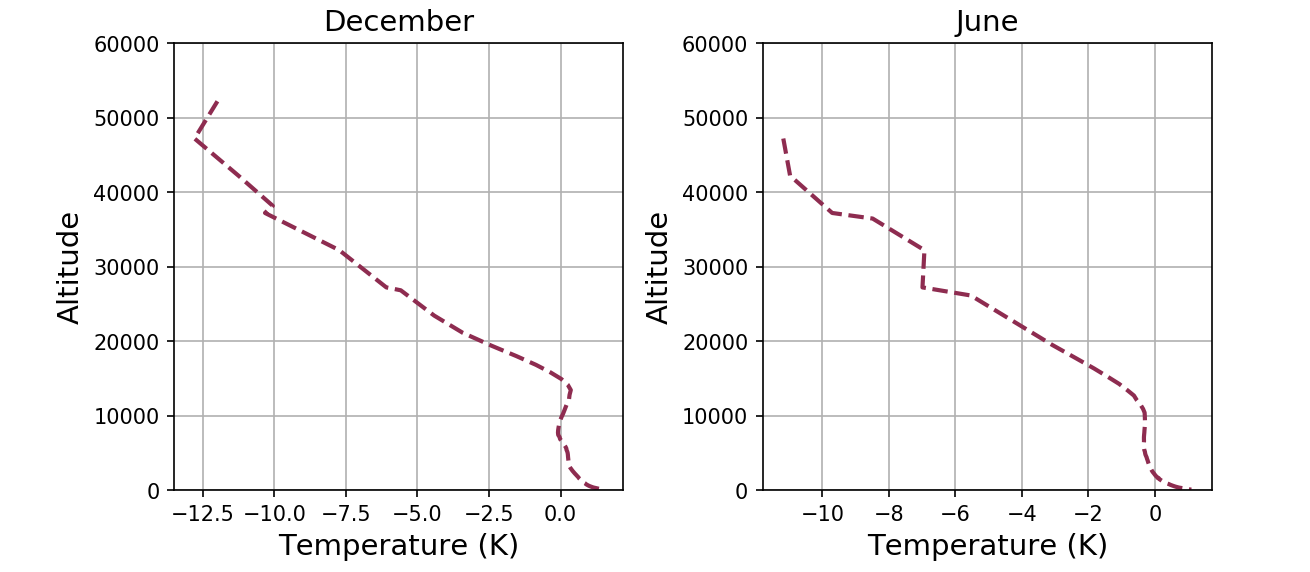
\includegraphics[width=.8\textwidth]{temp_evolution.png}
\centering
\caption{Temperature differences in December and June between the base and double \ce{CO_2} case (380ppm - 760ppm). We see increased stratospheric cooling and tropospheric warming in the double \ce{CO_2} case}
\label{fig:temp_step}
\end{figure}

We tested our interpretation by calculating the approximate pressure from which radiation would occur for an optical thickness of $\tau = 1$, assuming a \ce{CO_2} absorption coefficient of $\kappa = 1\; m^2/kg$ for a wavelength of 15 $\micro$m. This is an approximation, as the absorption coefficient varies with pressure and height, but it provides insight into the approximate radiating pressures. This is calculated by integrating $\text{d}\tau = \kappa q\,\text{d}p / g$ to $\tau = 1$, which gives
\begin{equation}
    P_{emis} = \frac{g}{\kappa q},
\end{equation}
where $g$ is gravitational acceleration, $q$ is the mass mixing ratio in ppm, and $\kappa$ is the absorption coefficient. We assume a column average $q$ and $\kappa$, rather than computing it separately for each pressure, temperature, and frequency. In this case, we find $P_{emis}$ to be 258 hPa and 129 hPa for the base case and double \ce{CO_2} case, respectively. This adequately explains why we see winter months decreasing in OLR as \ce{CO_2} concentration increases (Figure \ref{fig:init_OLR}), as the temperature at 129 hPa is lower than at 258 hPa (Figure \ref{fig:temperature_profiles}), while in the summer months the temperature at 129 hPa is greater than that at 258 hPa, which leads to our increased OLR.

\section{Discussion}
Under different \ce{CO_2} concentrations, at our model equilibrium, we find that the surface temperature warms an additional 1.1\degree  of warming during June, and an additional 1.5\degree  of warming in December due to a doubling of \ce{CO_2}. This supports previous work in the conclusion that diagnosing the sign of OLR cannot be used to immediately predict the surface level temperature response to GHG in the case of the Antarctic \citep{flanner_climate_2018}. Instead, it is necessary to look at the change in net surface flux to diagnose the response of surface temperatures to changing concentrations of \ce{CO_2}. 

OLR is also insufficient to understand the entire atmospheric response to changing GHG concentrations, as we find tropospheric warming due to increased \ce{CO_2}, but stratospheric cooling across all months. This column response is actually similar to that of locations where there is no temperature inversion, and in which OLR decreases in response to increases in \ce{CO_2} concentrations.

Surface albedo responses are not taken into account, nor are changes in atmospheric concentrations of absorbers, which will both change in response to a increasing surface temperatures and decreasing stratospheric temperatures. Additionally, our treatment of each month as a separate part of the model does not allow the conditions of a prior month to impact the conditions of the next month. Despite these limitations, our analysis provides insight into the response of a number of processes to changing concentrations in 
\ce{CO_2}.

\section{Acknowledgements}
I am really grateful for the advising of Tim Cronin on this project, and for the amount of time and effort he put in to helping me de-bug the model, while also taking the time to answer my questions on atmospheric radiation. Additional support came from the many students and postdocs in the atmospheric chemistry colloquium as well as PAOC who provided feedback on my presentation and paper. 
\pagebreak
\bibliographystyle{apalike}
\bibliography{references.bib}

\end{document}

